\section{Hybrid positioning}

The absolute positioning method is quit accurate but still it suffers from noise. On the other hand relative position has a lot uncertainty, because of the physical interference. By combing these two positioning methods we can get more precise location based on sensor measurements from absolute and prediction from the relative positions. This combination is called hybrid positioning. One of the methods achieving hybrid position is with Kalman filter, which will be described below.

\subsection{Kalman filter}

The Kalman filter was made by Rudolf E. Kalman. It was developed for Apollo mission to the moon, to track the location of the space shuttle. This method is still used, because it dos not require a lot of processing power and memory space. The reasoning is that the method dos not need to save any data apart the model of movement and and previews position.

The process of the filter is as follow:
\begin{enumerate}
	\item Predict the position form previews position and movement of the model
	\item Correct the position with the measured data
	\item Repeat step 1 and 2
\end{enumerate}

Fidure\ref{fig:KalmanfilterRotation} shows it visually.

\begin{figure}[H]
	\centering
	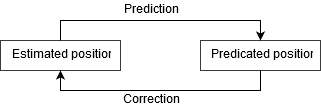
\includegraphics[width=0.4\linewidth]{positioning/positioning/KalmanFilterProcess}
	\caption{Kalmans filter principal}
	\label{fig:KalmanfilterRotation}
\end{figure}

In the Figure\ref{fig:Kalmanfilter} is displayed two case how the filter works. First one is when time(T-1) and time(T). In this case the filter goes closer to the measurement Gaussian, because it is more reliable.The hybrid position probability is higher then absolute and relative positioning this is because the absolute and relative position Gaussian's are multiplied together. The second case is in the period (T) and (T+1) in this case the measurements has a lot more noise in them. Then the estimation is moving further from the measurement Gaussian, because of the lower probability. 

\begin{figure}[H]
	\centering
	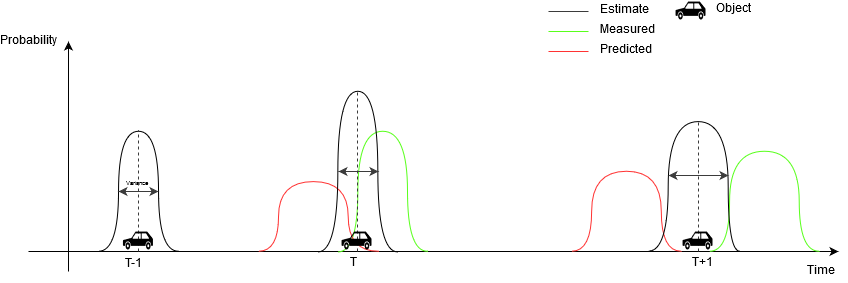
\includegraphics[width=0.7\linewidth]{positioning/positioning/DiagramKalman}
	\caption{Kalmans filter example}
	\label{fig:Kalmanfilter}
\end{figure}